

\textbf{Цель работы}: исследование системы автоматической посадки самолета по глиссаде с помощью математического моделирования на персональном компьютере. Рассматривается плоская задача продольного движения. Работа содержит:
\begin{itemize}
    \item \textbf{Лабораторная работа №3. Исследования системы автоматической посадки самолета при позиционном регуляторе в контуре глиссады.}
    \item \textbf{Лабораторная работа №4. Исследование системы автоматической посадки самолета при форсирующем регуляторе в контуре глиссады.}
\end{itemize}

\section{Теоретический минимум}

Полет по глиссаде начинается с момента прохождения самолетом  точки 1 на рис.\ref{fig:Полёт по глисаде} С этого момента начинается снижение самолета по сигналам глиссадного маяка до высоты порядка 20 м, пока имеется устойчивый сигнал глиссадного радиомаяка (ГРМ). Стабилизация самолета относительно глиссады в этом случае производится путем изменения угла тангажа самолета. Это обеспечивается каналом руля высоты.

\begin{figure}[H]
    \center{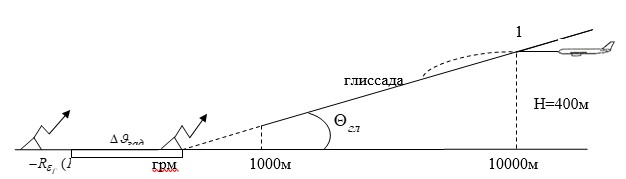
\includegraphics[width=\linewidth]{figures/1.jpg}}
    \caption{Полёт по глисаде}
    \label{fig:Полёт по глисаде}
\end{figure}

При полете по глиссаде самолет должен снижаться с постоянной скоростью. Выполнение этого требования возлагается на автомат тяги, который стабилизирует заданное значение скорости.

Схема аппаратурного построения канала руля высоты системы автоматической посадки по глиссаде приведена на рис. \ref{fig:Cистема автоматической посадки по глиссаде}

\begin{figure}[H]
    \center{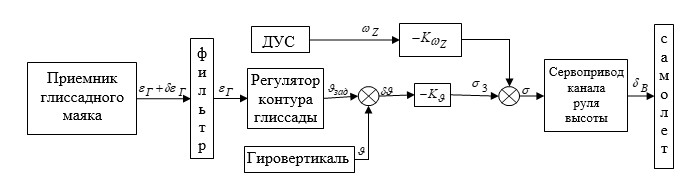
\includegraphics[width=\linewidth]{figures/2.jpg}}
    \caption{Cистема автоматической посадки по глиссаде}
    \label{fig:Cистема автоматической посадки по глиссаде}
\end{figure}

Для формирования контура управления продольным движением при полете самолета по глиссаде рассмотрим геометрию движения по радиолучу (рис. \ref{fig:Полёт по глисаде 2}). Из рис. \ref{fig:Полёт по глисаде 2} видно, что $\varepsilon_\text{Г} = \frac{d}{D} $ и $\dot{d} = V\Delta \theta$. Отсюда находим связь между $\varepsilon_\text{Г}$ и $\Delta \theta$. Проводя преобразования Лапласа, при замороженном значении дальности $D$ получаем:

$$ \varepsilon_\text{Г} = \frac{V}{D} \cdot \frac{1}{p} \cdot \Delta \theta  $$

\begin{figure}[H]
    \center{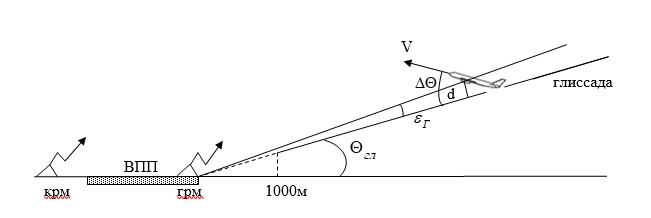
\includegraphics[width=\linewidth]{figures/3.jpg}}
    \caption{Полёт по глисаде}
    \label{fig:Полёт по глисаде 2}
\end{figure}

С учетом полученного соотношения структурная схема контура управления движением самолета по глиссаде в пренебрежении динамикой измерителей и сервопривода принимает вид, приведенный на рис. \ref{fig:Cистема автоматической посадки по глиссаде 2}. Введение внутренних контуров по угловой скорости $\omega_z$ и углу тангажа $\vartheta$  позволяет улучшить характеристики устойчивости и управляемости самолета, т.е. улучшить динамические характеристики самолета и расширить область возможных частот управления.

\begin{figure}[H]
    \center{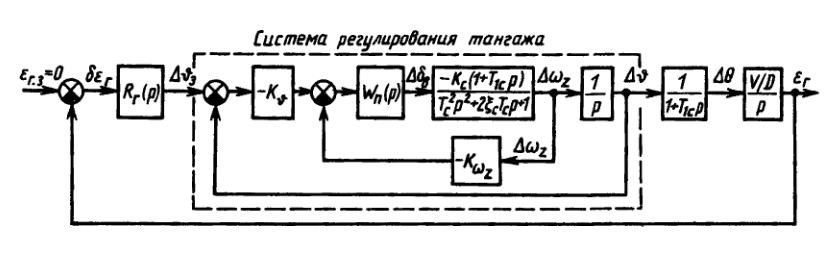
\includegraphics[width=\linewidth]{figures/6.jpg}}
    \caption{Структурная схема стабилизации глиссады}
    \label{fig:Cистема автоматической посадки по глиссаде 2}
\end{figure}

\section{Модель исследуемой системы}
\label{eq: СДУ}
\begin{equation}
    \begin{cases}
    \dot{\omega_z} = K_{z}m_z^{\bar{\omega}_z}\frac{b_a}{V} \omega_z + K_z m_z^{\alpha} \alpha + K_z m_z^{\dot{\alpha}} \frac{b_a}{V} \dot{\alpha} + K_z m_z^{\delta_\text{в}}\delta_\text{в}\\
    \dot{\alpha} = \omega_z - \bar{Y}^\alpha \alpha \\ 
    \dot{\vartheta} = \omega_z \\ 
    \dot{V_y} = V \cdot \bar{Y}^\alpha\alpha
\end{cases}
\end{equation}

При исследовании автоматической посадки самолета эту систему необходимо дополнить кинематическим уравнением для угла $\varepsilon_{\text{Г}}$:
$$\dot{\varepsilon_\text{Г}}=\frac{V}{D} \theta$$
и угла наклона траектории:
$$\theta = \vartheta - \alpha$$.

Кроме того, вводятся уравнения автопилота, выражающие закон управления рулем высоты:

\begin{equation}
    \delta_B = K_{\omega_z} \omega_z - K_{\vartheta}(\vartheta_{\text{зад}}-\vartheta) \\ 
\end{equation}
$$\delta_\text{зад} = -(K_{\varepsilon_\text{Г}}\varepsilon_\text{Г}+K_{\dot{\varepsilon}_\text{Г}}\dot{\varepsilon}_\text{Г})$$

\section{Исходные данные}

\begin{table}[H]
    \centering
    \caption{Таблица исходных данных}
    \begin{tabular}{|c|c|}
    \hline
        Параметр& Значение \\ \hline
        $a_1,1/c$&0,75 \\ \hline
        $a_2, 1/c^2$&5,5 \\ \hline
        $a_3, 1/c^2$& 4\\ \hline
        $a_4, 1/c^$& 1\\ \hline
        $a_5, 1/c^$& 0,25\\ \hline
        $V, $м/c&60 \\ \hline
        $K_{\omega_z}, c$&0,68 \\ \hline
        $K_\vartheta$& 2,01\\ \hline
        $\tau_1$& 1,83\\ \hline
        $\tau_2$& 0,26\\ \hline
        $\xi_2$&0,54 \\ \hline
    \end{tabular}
    \label{tab:my_label}
\end{table}

\begin{table}[H]
    \centering
    \caption{Таблица исходных данных по высоте и дальности}
    \begin{tabular}{|c|c|c|c|c|c|}
    \hline
        Дальность, м & 10000 & 8000 & 4000 & 2000 & 1000 \\ \hline
        Высота, м & 400 & 320 & 160 & 80 & 40\\ \hline
    \end{tabular}
    \label{tab:InitialData}
\end{table}

\section{Выполнение работы}

\begin{center}
    \subsection*{\underline{ Лабораторная работа №3.} Выбор значений коэффициента $K_{\varepsilon_\text{Г}}$
позиционного регулятора.}
\end{center}

\begin{table}[H]
    \centering
    \caption{Результаты моделирования для дальности 10 км}
    \begin{tabular}{c|c|c|c|c|c|c}
    \hline
        $K_{\varepsilon_\text{Г}}$& 20  & 22,77 & 24 & 25 & 27 &\cellcolor{cyan}28\\ \hline
        $t_\text{рег}$& 20 & 16,5 & 15,5 & 14,5 & 13,3 &\cellcolor{cyan}12,5\\ \hline
        Процесс& Aпер. & Aпер. & Aпер. & Aпер. & Aпер. &\cellcolor{cyan}Aпер.\\ \hline
    \end{tabular}
    \label{tab:10KM}
\end{table}

\begin{table}[H]
    \centering
    \caption{Результаты моделирования для дальности 8 км}
    \begin{tabular}{c|c|c|c|c|c|c}
    \hline
        $K_{\varepsilon_\text{Г}}$& 17  & 18 & 19& 20 & 21 &\cellcolor{cyan}22\\ \hline
        $t_\text{рег}$& 18 & 16,75 & 15,5 & 14,5 & 13,7 &\cellcolor{cyan}13\\ \hline
        Процесс& Aпер. & Aпер. & Aпер. & Aпер. & Aпер. &\cellcolor{cyan}Aпер.\\ \hline
    \end{tabular}
    \label{tab:10KM}
\end{table}

\begin{table}[H]
    \centering
    \caption{Результаты моделирования для дальности 4 км}
    \begin{tabular}{c|c|c|c|c|c|c}
    \hline
        $K_{\varepsilon_\text{Г}}$& 7  & 10 & \cellcolor{cyan}11 & 12 & 20 &30\\ \hline
        $t_\text{рег}$& 23 & 14,5 & \cellcolor{cyan}13 & 11,5 & 13,2 &11\\ \hline
        Процесс& Aпер. & Aпер. & \cellcolor{cyan}Aпер. & Кол. & Кол. &Кол.\\ \hline
    \end{tabular}
    \label{tab:10KM}
\end{table}

\begin{table}[H]
    \centering
    \caption{Результаты моделирования для дальности 2 км}
    \begin{tabular}{c|c|c|c|c|c|c}
    \hline
        $K_{\varepsilon_\text{Г}}$& 3  & 4 & \cellcolor{cyan}5 & 6 & 7 &8\\ \hline
        $t_\text{рег}$& 27 & 19 & \cellcolor{cyan}14,5 & 11,5 & 9,6 &8,3\\ \hline
        Процесс& Aпер. & Aпер. &\cellcolor{cyan} Aпер. & Кол. & Кол. &Кол.\\ \hline
    \end{tabular}
    \label{tab:10KM}
\end{table}

\begin{table}[H]
    \centering
    \caption{Результаты моделирования для дальности 1 км}
    \begin{tabular}{c|c|c|c|c|c|c}
    \hline
        $K_{\varepsilon_\text{Г}}$& 3 & 4 & 2,6 & 2,5 & \cellcolor{cyan}2,8 &2,7\\ \hline
        $t_\text{рег}$& 11,5& 8,4& 13,8 & 14,5 & \cellcolor{cyan}12,5 &13,2\\ \hline
        Процесс& Кол. & Кол. & Aпер. & Апер. & \cellcolor{cyan}Апер. &Апер.\\ \hline
    \end{tabular}
    \label{tab:10KM}
\end{table}

\begin{figure}[H]
    \centering
    \center{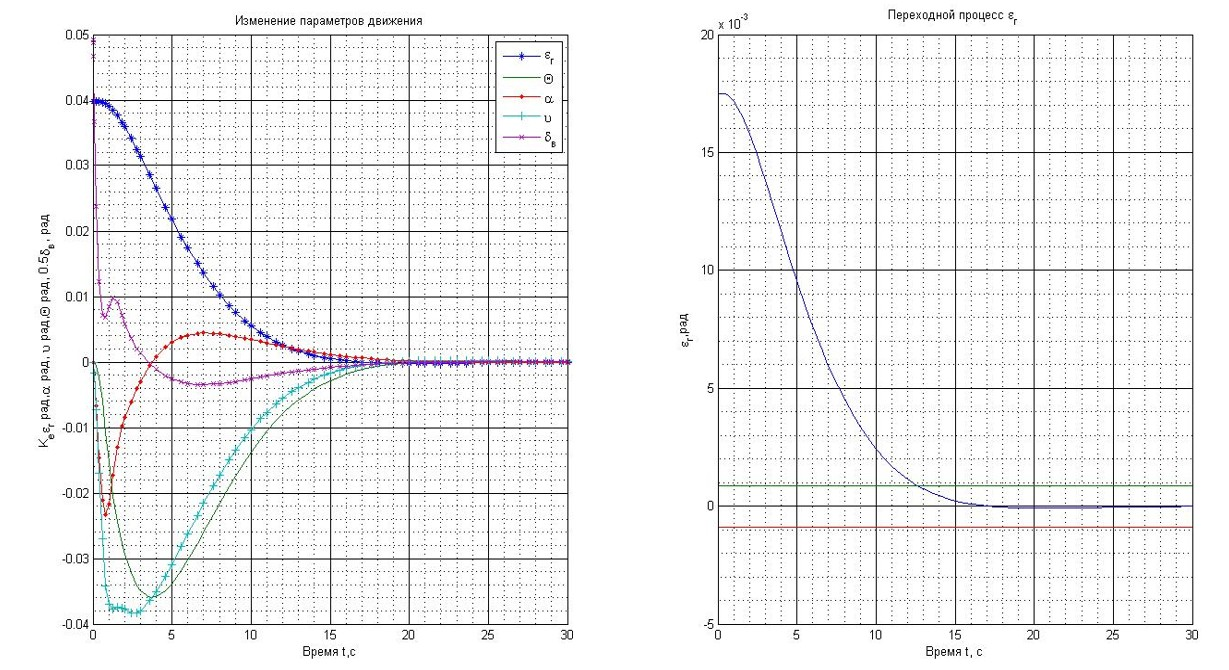
\includegraphics[width=\linewidth]{figures/4.jpg}}
    \caption{График переходных процессов}
    \label{fig:steps}
\end{figure}

\begin{table}[H]
    \centering
    \begin{tabular}{c|c|c|c|c|c}
    \hline
        $D$, м & 10 000 & 8000 & 4000 & 2000 & 1000  \\ \hline
        $H$, м & 400 & 320 & 160 & 80 & 40  \\ \hline
        $K_{\xi_\text{Г}} \approx$ & 22,77 & 18,215 & 9,1 & 4,55 & 2,27  \\ \hline
        $K_{\xi_\text{Г}_{max}}$ & 91 & 72,86 & 36,43 & 18,2 & 9,1  \\ \hline
        $K_{\xi_\text{Г}_\text{опт}}$ & 28 & 22 & 11 & 5 & 2,8  \\ \hline
        $t_\text{рег},$ c & 12,6 & 13 & 13 & 14,5 & 12,5  \\ \hline
    \end{tabular}
\end{table}

\begin{center}
    \subsection*{\underline{ Лабораторная работа №4.} Выбор значений коэффициента $K_{\varepsilon_\text{Г}} \  \text{и} \  K_{\dot{\varepsilon}_\text{Г}}$
позиционного регулятора.}
\end{center}

\begin{table}[H]
    \centering
    \caption{Результаты моделирования для дальности 10 км}
    \begin{tabular}{c|c|c|c|c|c|c}
    \hline
        $K_{\varepsilon_\text{Г}}$ & 160 & 165 &\cellcolor{cyan} 200 & 161 & 300 & 180  \\ \hline
        $t_\text{рег}$ & 6,8 & 6,75 &\cellcolor{cyan} 6,6 & 7 & 6 & 6,7  \\ \hline
        Процесс & Aпер. & Aпер. & \cellcolor{cyan}Aпер. & Aпер. & Кол. & Aпер.  \\ \hline
    \end{tabular}
    \label{tab:10KM}
\end{table}

\begin{table}[H]
    \centering
    \caption{Результаты моделирования для дальности 8 км}
    \begin{tabular}{c|c|c|c|c|c|c}
    \hline
        $K_{\varepsilon_\text{Г}}$& 125 & 128 & 130 & 150 & \cellcolor{cyan}170 & 160  \\ \hline
        $t_\text{рег}$ & 7 & 7 & 6,8 & 6,65 & \cellcolor{cyan}6,5 & 6,6  \\ \hline
        Процесс& Aпер. & Aпер. & Aпер. & Aпер. & \cellcolor{cyan}Aпер. &Aпер.\\ \hline
    \end{tabular}
    \label{tab:10KM}
\end{table}

\begin{table}[H]
    \centering
    \caption{Результаты моделирования для дальности 4 км}
    \begin{tabular}{c|c|c|c|c|c|c}
    \hline
        $K_{\varepsilon_\text{Г}}$& 60 & 65 & 80 & \cellcolor{cyan}90 & 70 & 85  \\ \hline
        $t_\text{рег}$ & 7 & 6,8 & 6,6 &\cellcolor{cyan} 6,4 & 6,7 & 6,5  \\ \hline
        Процесс& Aпер. & Aпер. & Aпер. &\cellcolor{cyan} Aпер. & Aпер. &Aпер.\\ \hline
    \end{tabular}
    \label{tab:10KM}
\end{table}

\begin{table}[H]
    \centering
    \caption{Результаты моделирования для дальности 2 км}
    \begin{tabular}{c|c|c|c|c|c|c}
    \hline
        $K_{\varepsilon_\text{Г}}$& 20 & 30 & 40 & \cellcolor{cyan}45 & 35 & 50  \\ \hline
        $t_\text{рег}$ & 8 & 7,0 & 6,6 & \cellcolor{cyan}6,5 & 6,7 & 6,3  \\ \hline
        Процесс& Aпер. & Aпер. & Aпер. &\cellcolor{cyan} Aпер. & Aпер. &Кол.\\ \hline
    \end{tabular}
    \label{tab:10KM}
\end{table}

\begin{table}[H]
    \centering
    \caption{Результаты моделирования для дальности 1 км}
    \begin{tabular}{c|c|c|c|c|c|c}
    \hline
        $K_{\varepsilon_\text{Г}}$& 10 & 15 & 20 & \cellcolor{cyan}25 & 30 & 40  \\ \hline
        $t_\text{рег}$ & 8,1 & 7,0 & 6,6 &\cellcolor{cyan} 6,3 & 6 & 5,5  \\ \hline
        Процесс& Кол. & Кол. & Aпер. &\cellcolor{cyan} Апер. & Кол. &Кол.\\ \hline
    \end{tabular}
    \label{tab:10KM}
\end{table}

\begin{figure}[H]
    \centering
    \center{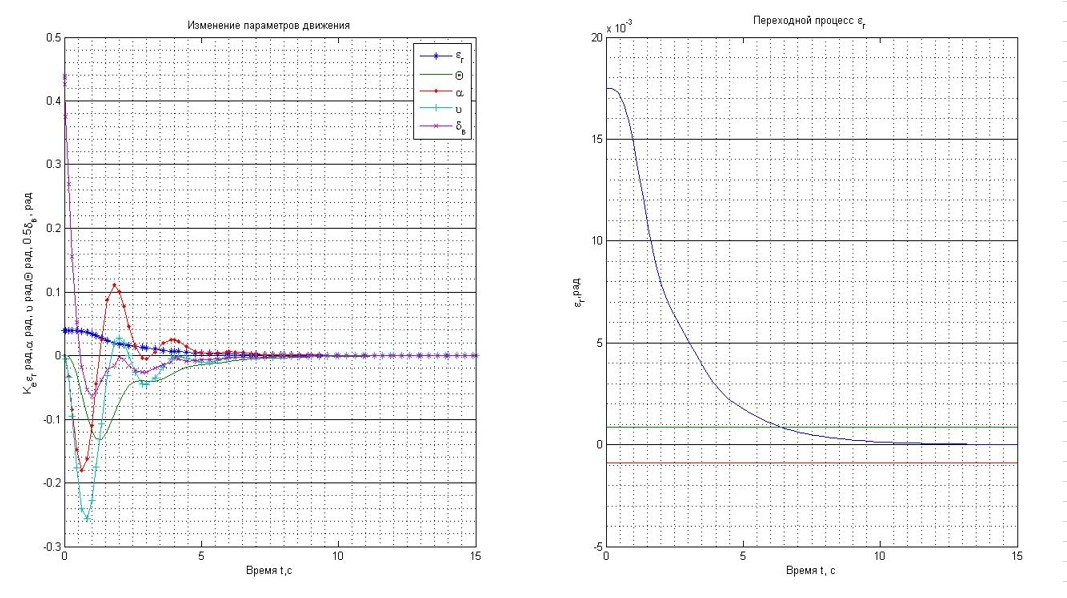
\includegraphics[width=\linewidth]{figures/5.jpg}}
    \caption{График переходных процессов}
    \label{fig:steps2}
\end{figure}

\begin{table}[H]
    \centering
    \begin{tabular}{c|c|c|c|c|c}
    \hline
        $D$, м & 10 000 & 8000 & 4000 & 2000 & 1000  \\ \hline
        $H$, м & 400 & 320 & 160 & 80 & 40  \\ \hline
        $K_{\xi_\text{Г}} \approx$ &160,26 & 128,2 & 64,1 & 32,05 & 16,02  \\ \hline  
        $K_{\xi_\text{Г}_{max}}$ & 641 & 512,8 & 256,4 & 128,2 & 64,1  \\ \hline
        $K_{\xi_\text{Г}_\text{опт}}$ &200 & 170 & 90 & 45 & 25  \\ \hline
        $K_{\dot{\xi}_\text{Г}_\text{опт}}$ & 366 & 311,1 & 164,7 & 82,35 & 45,75  \\ \hline
        $t_\text{рег},$ c & 6,6 & 6,5 & 6,4 & 6,5 & 6,3  \\ \hline
    \end{tabular}
\end{table}

\begin{center}
    \item \section*{Выводы}
\end{center}
\begin{enumerate}
    \item При уменьшении дальности до ГРМ и высоты полета коэффициенты как позиционного регулятора, так и форсирующего регулятора уменьшаются.
    \item При введении форсирующего регулятора время регулирования переходного процесса по отклонению от глиссады уменьшилось практически в 2 раза, так как при форсирующем регуляторе в системе учитывается не только величина сигнала отклонения от глиссады, но и скорость его изменения.
    \item При замене позиционного звена форсирующим время регулирования переходных процессов по углу атаки, углу тангажа и т.д. также уменьшилось более чем в 2 раза, но переходные процессы стали более колебательными, кроме переходного процесса величины отклонения от глиссады, данный процесс апериодический, чего и требовалось достичь.
    \item При введении форсирующего регулятора наименьшее время регулирования составило 6,3 с среднее время на всех дальностях около 6 с. Оптимальные значения коэффициентов $K_{\xi_\text{Г}_\text{опт}_\text{ф}}$ и $K_{\dot{\xi}_\text{Г}_\text{опт}_\text{ф}}$ изменяются на всем диапазоне дальностей от 25 до 200, от 45,75 до 366 соответственно.
    \item При введении позиционного регулятора наименьшее время регулирования составило 12,5 с среднее время на всех дальностях около 13 с. Оптимальные значения коэффициента  $K_{\dot{\xi}_\text{Г}}$ изменяются на всем диапазоне дальностей от 2,8 до 28.
\end{enumerate}

\begin{center}
    \item \section*{Контрольные вопросы}
\end{center}

\begin{enumerate}
    \item Чем объясняется потребность и в чем особенность автоматизации этапа посадки?
    \item Как осуществляется построение контура стабилизации глиссады? В чем его особенность?
    \item Для чего в контур стабилизации глиссады вводятся внутренние контуры демпфирования и стабилизации угла тангажа?
    \item Какие по структуре регуляторы вводятся в контур стабилизации глиссады? Почему?
    \item Каков характер изменения коэффициентов регулятора от высоты (дальности до ГРМ) снижения самолета по глиссаде?
\end{enumerate}

\textbf{Ответы:}

\begin{enumerate}
    \item Одной из важнейших проблем развития авиации является обеспечение безопасности и регулярности полетов. В гражданской авиации от решения этой проблемы зависит соблюдение графика полетов самолетов и экономическая эффективность их использования. Для того чтобы увеличить регулярность и безопасность полетов вводится автоматизация этапа посадки, благодаря ней можно совершать посадку в сложных погодных условиях, также она снижает вероятность ошибки летчика из-за недостатка опыта совершения посадки. При проектировании систем автоматизации посадки большое внимание необходимо уделять времени регулирования, оно должно быть минимальным, так при посадке самолет теряет высоты и необходимо большое быстродействие системы. 
    \item Стабилизация самолета относительно глиссады производится путем изменения угла тангажа самолета. Это обеспечивается каналом руля высоты. На радиоприемник от ГРМ поступает сигнал отклонения от заданной линии глиссады далее сигнал проходит через фильтры и идет в систему и при помощи позиционного или форсирующего регулятора сигнал деформируется и идет далее в АП тангажа , после этого сигнал идет в обратную связь, таким образом стабилизируется до заданного значения. Особенность такого контура в том, что он неустойчив без внутренних обратных связей.
    \item Если не вводить дополнительные внутренние обратные связи, в разомкнутой цепи системы появится астатизм второго порядка, что приведет к неустойчивости системы.
    \item Существует два вида регуляторов это позиционный и форсирующий. Позиционный представляет из себя коэффициент усиления, с ним система хорошо работает, но быстродействие все же мало. Для увеличения быстродействия применяют форсирующий регулятор, так как с ним в системе учитывается не только величина отклонения от глиссады, но и её изменение с течением времени. Введение сигнала производной расширяет область устойчивости по коэффициенту $K_{\dot{\xi}_\text{Г}}$, что позволяет выбрать бóльшее усиление, чем в случае позиционного регулятора, и тем самым уменьшить время регулирования.
    \item При уменьшении дальности до ГРМ (высоты) коэффициенты как позиционного регулятора, так и форсирующего уменьшаются, причем довольно значительно, это можно пронаблюдать по ранее приведенным графикам данной работы.  
\end{enumerate}

